\documentclass[xetex,mathserif,serif]{beamer}
\usepackage{polyglossia}
\setdefaultlanguage[babelshorthands=true]{russian}
\usepackage{minted}
\usepackage{tabu}

\useoutertheme{infolines}

\usepackage{fontspec}
\setmainfont{FreeSans}
\newfontfamily{\russianfonttt}{FreeSans}

\usepackage{textpos}
\setlength{\TPHorizModule}{1cm}
\setlength{\TPVertModule}{1cm}

\setbeamertemplate{blocks}[rounded][shadow=false]

\setbeamercolor*{block title alerted}{fg=red!50!black,bg=red!20}
\setbeamercolor*{block body alerted}{fg=black,bg=red!10}

\tabulinesep=1.2mm

\title{Занятие 12: Continuous Delivery}
\author[Юрий Литвинов]{Юрий Литвинов\\\small{\textcolor{gray}{yurii.litvinov@gmail.com}}}
\date{29.11.2017}

\newcommand{\todo}[1] {
	\begin{center}\textcolor{red}{TODO: #1}\end{center}
}

\newcommand{\DownArrow} {
	\hspace{2cm}\begin{LARGE}$\downarrow$\end{LARGE}
}

\newcommand{\attribution}[1] {
	\begin{flushright}\begin{scriptsize}\textcolor{gray}{\textcopyright\; #1}\end{scriptsize}\end{flushright}
}

\begin{document}

	\frame{\titlepage}

	\begin{frame}
		\frametitle{Docker}
		\begin{center}
			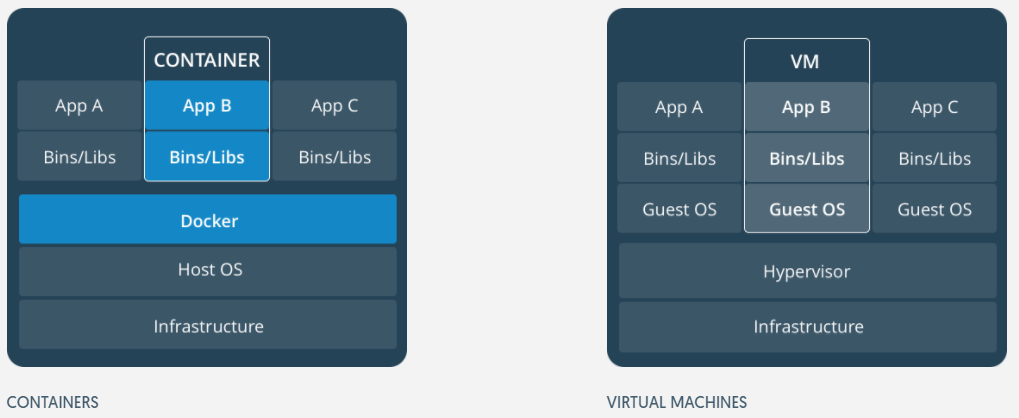
\includegraphics[width=\textwidth]{docker.png}
			\attribution{\url{https://www.docker.com}}
		\end{center}
	\end{frame}
	
	\begin{frame}[fragile]
		\frametitle{Dockerfile}
		\begin{scriptsize}
			\begin{minted}{sh}
# Use an official Python runtime as a parent image
FROM python:2.7-slim

# Set the working directory to /app
WORKDIR /app

# Copy the current directory contents into the container at /app
ADD . /app

# Install any needed packages specified in requirements.txt
RUN pip install --trusted-host pypi.python.org -r requirements.txt

# Make port 80 available to the world outside this container
EXPOSE 80

# Define environment variable
ENV NAME World

# Run app.py when the container launches
CMD ["python", "app.py"]
			\end{minted}
		\end{scriptsize}
	\end{frame}

	\begin{frame}[fragile]
		\frametitle{Балансировка нагрузки}
		\framesubtitle{docker-compose.yml}
		\begin{scriptsize}
			\begin{minted}{yaml}
version: "3"
services:
    web:
        # replace username/repo:tag with your name and image details
        image: username/repo:tag
        deploy:
            replicas: 5
            resources:
                limits:
                    cpus: "0.1"
                    memory: 50M
            restart_policy:
                condition: on-failure
        ports:
            - "80:80"
        networks:
            - webnet
networks:
    webnet:
			\end{minted}
		\end{scriptsize}
	\end{frame}

	\begin{frame}
		\frametitle{Swarm-ы}
		\begin{center}
			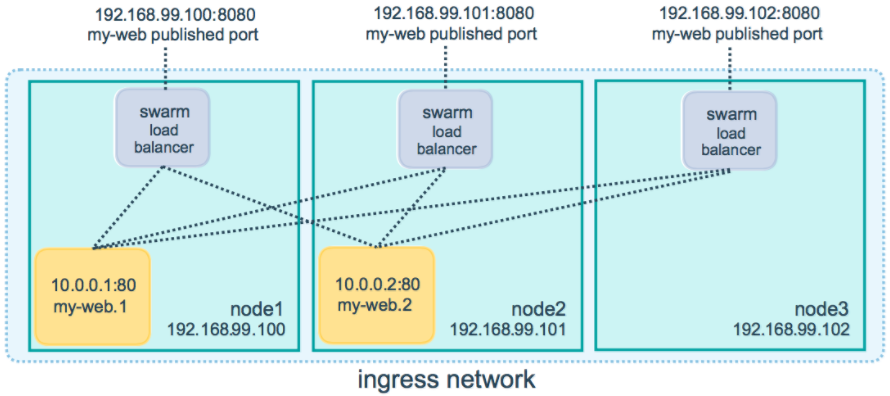
\includegraphics[width=\textwidth]{swarmLoadBalancing.png}
			\attribution{\url{https://www.docker.com}}
		\end{center}
	\end{frame}

	\begin{frame}
		\frametitle{Сборка в Docker}
		\begin{itemize}
			\item Приложение: \url{https://github.com/trikset/trikRuntime}
			\begin{itemize}
				\item Прошивка для робота, C++ с Qt
			\end{itemize}
			\item Dockerfile: \url{https://github.com/trikset/trikRuntime/blob/master/docker/Dockerfile}
			\item .travis.yml: \url{https://github.com/trikset/trikRuntime/blob/master/.travis.yml}
		\end{itemize}
	\end{frame}

	\begin{frame}
		\frametitle{Jenkins}
		\begin{itemize}
			\item Continuous Delivery-система
			\begin{itemize}
				\item Похожа на Travis, но более конфигурируема
			\end{itemize}
			\item Работает локально
			\begin{itemize}
				\item Следовательно, требует настройки и хостинга
				\item Следовательно, может использоваться в корпоративном окружении
			\end{itemize}
			\item Имеет кучу плагинов на все случаи жизни
			\item Опенсорсный, очень популярен по сей день
			\begin{itemize}
				\item Начинался в 2005 в Sun как Hudson
			\end{itemize}
		\end{itemize}
	\end{frame}

	\begin{frame}[fragile]
		\frametitle{Jenkinsfile}
		\begin{minted}{groovy}
pipeline {
    agent any
    stages {
        stage('build') {
            steps {
                sh 'mvn --version'
            }
        }
    }
}
		\end{minted}
	\end{frame}

	\begin{frame}[fragile]
		\frametitle{Более продвинутые шаги}
		\begin{minted}{groovy}
pipeline {
    agent any
    stages {
        stage('Deploy') {
            steps {
                retry(3) {
                    sh './flakey-deploy.sh'
                }

                timeout(time: 3, unit: 'MINUTES') {
                    sh './health-check.sh'
                }
            }
        }
    }
}
		\end{minted}
	\end{frame}

	\begin{frame}[fragile]
		\frametitle{Jenkins и Docker}
		\begin{minted}{groovy}
pipeline {
    agent { docker 'maven:3.5.2-jdk-8-slim' }
    stages {
        stage('build') {
            steps {
                bat 'mvn --version'
            }
        }
    }
}
		\end{minted}
	\end{frame}

	\begin{frame}[fragile]
		\frametitle{Переменные окружения}
		\begin{footnotesize}
			\begin{minted}{groovy}
pipeline {
    agent any

    environment {
        DB_ENGINE    = 'sqlite'
        AWS_ACCESS_KEY_ID     = credentials('AWS_ACCESS_KEY_ID')
        AWS_SECRET_ACCESS_KEY = credentials('AWS_SECRET_ACCESS_KEY')
    }

    stages {
        stage('Build') {
            steps {
                sh 'printenv'
            }
        }
    }
}
			\end{minted}
		\end{footnotesize}
	\end{frame}

	\begin{frame}[fragile]
		\frametitle{Слежение за тестами}
		\begin{minted}{groovy}
pipeline {
    agent any
    stages {
        stage('Test') {
            steps {
                sh './gradlew check'
            }
        }
    }
    post {
        always {
            junit 'build/reports/**/*.xml'
        }
    }
}
		\end{minted}
	\end{frame}

	\begin{frame}[fragile]
		\frametitle{Деплой, ручное подтверждение}
		\begin{scriptsize}
			\begin{minted}{groovy}
pipeline {
    agent any
    stages {
        ...
        stage('Deploy - Staging') {
            steps {
                sh './deploy staging'
                sh './run-smoke-tests'
            }
        }
        stage('Sanity check') {
            steps {
                input "Does the staging environment look ok?"
            }
        }
        stage('Deploy - Production') {
            steps {
                sh './deploy production'
            }
        }
    }
}
			\end{minted}
		\end{scriptsize}
	\end{frame}

	\begin{frame}
		\frametitle{Jenkins Blue Ocean}
		\begin{center}
			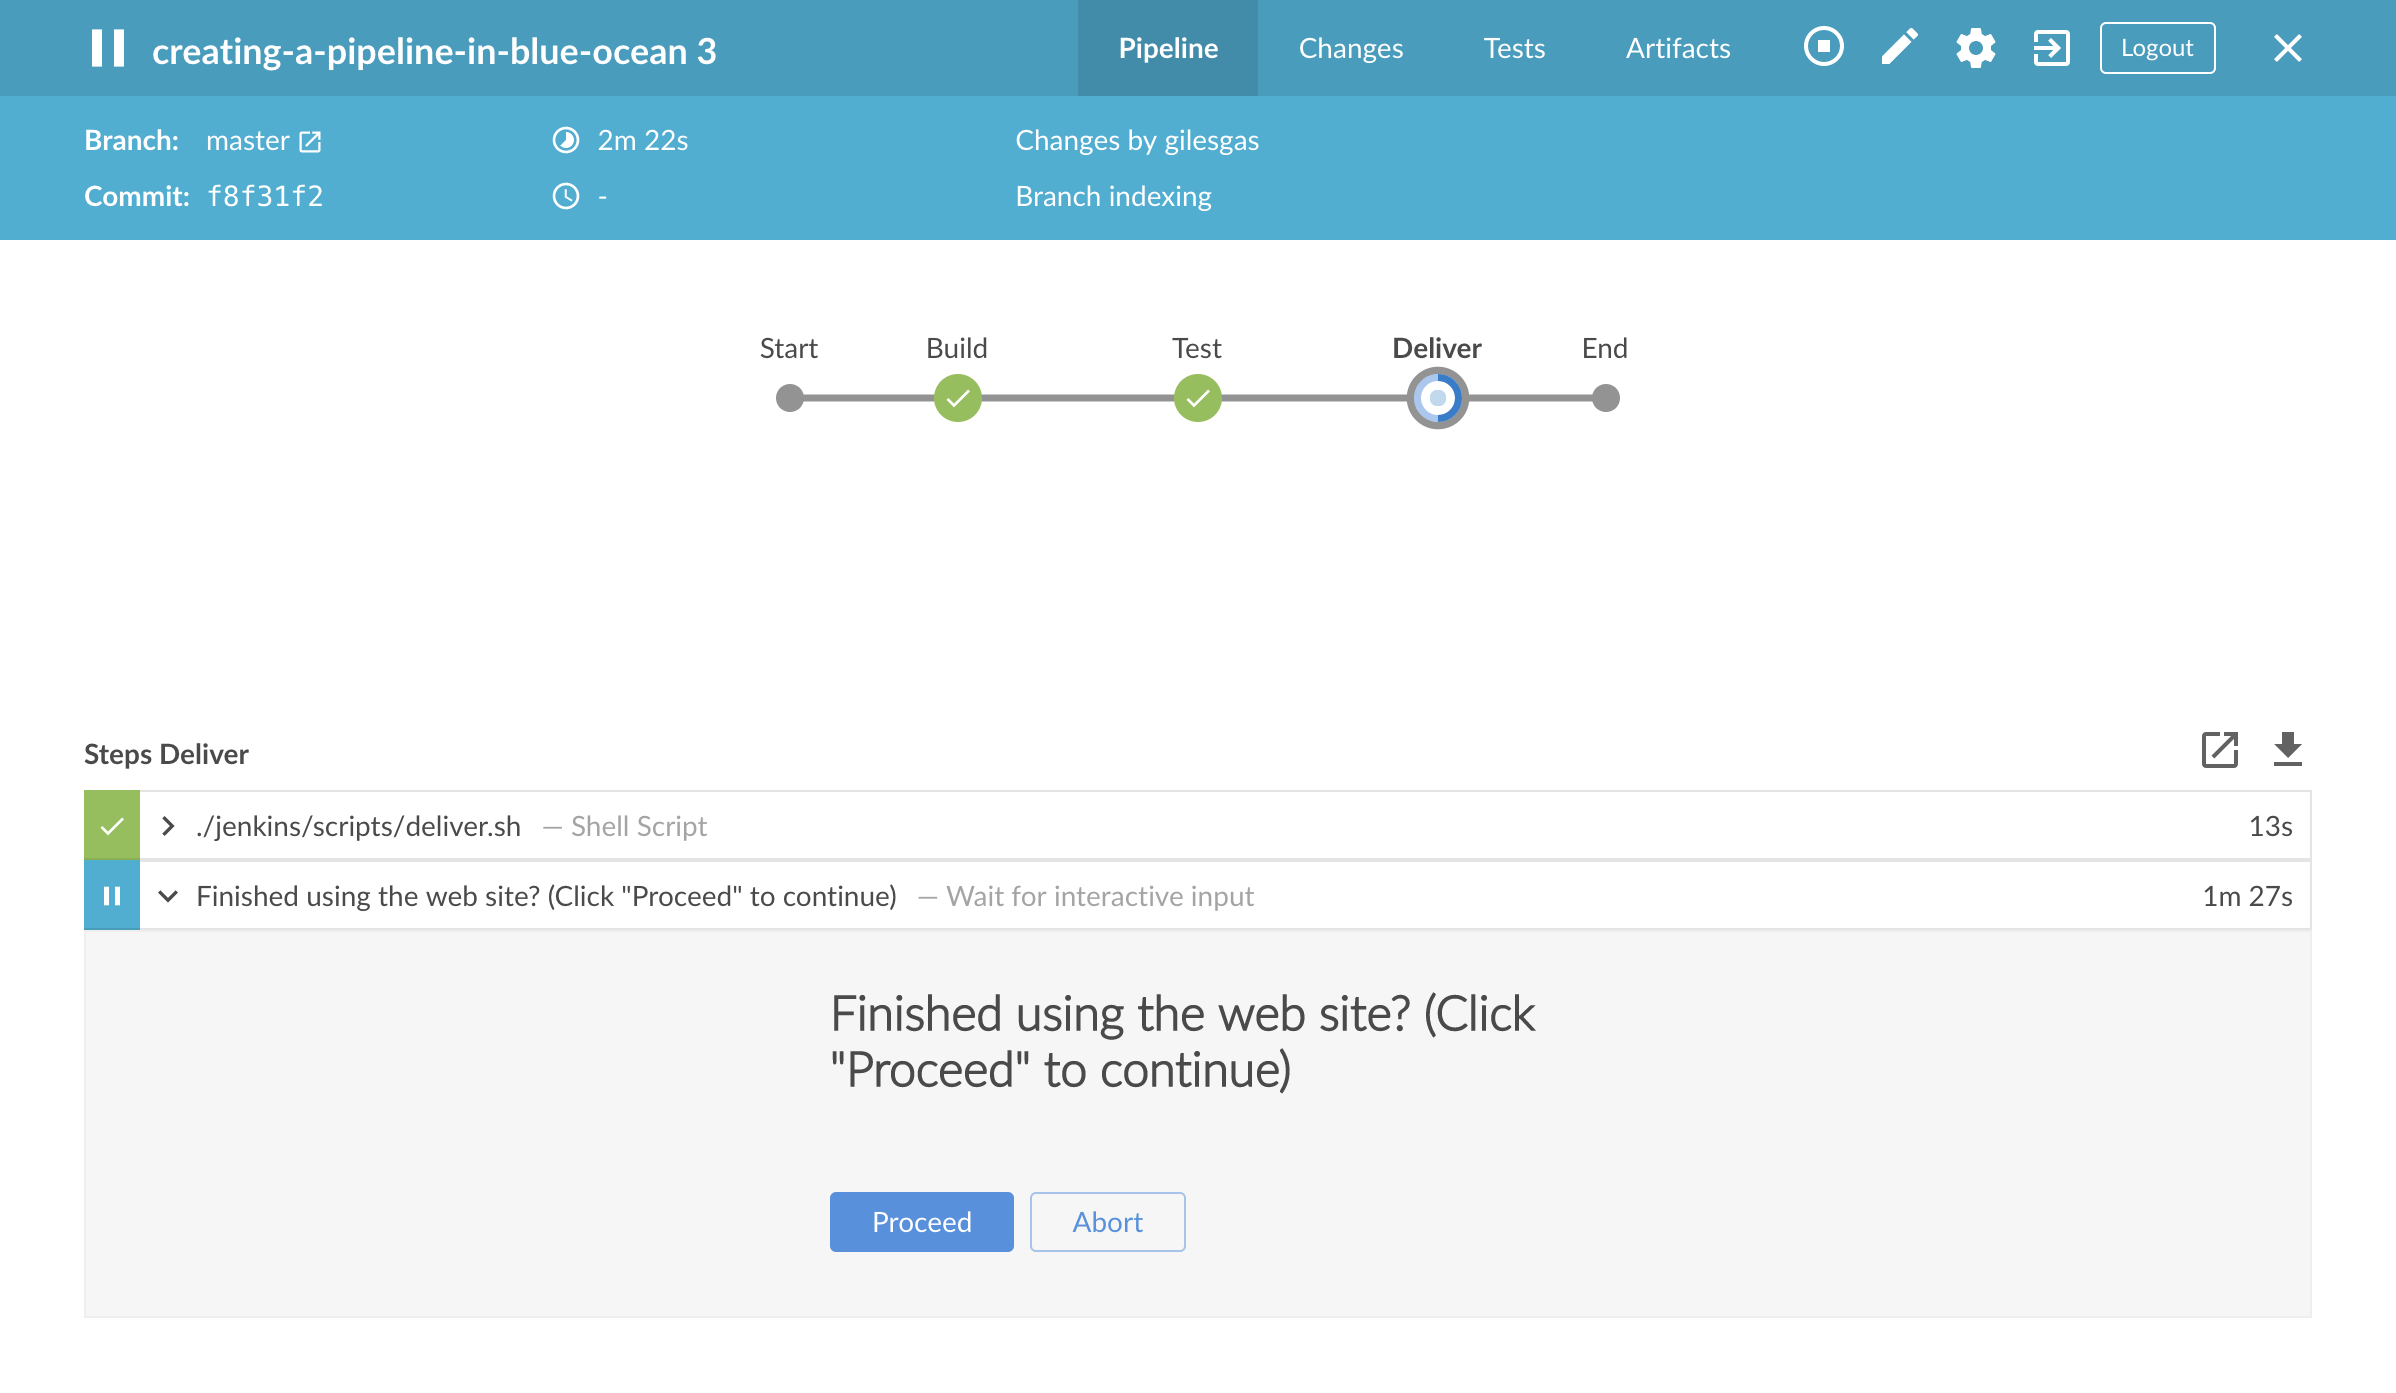
\includegraphics[width=0.8\textwidth]{blueOcean.png}
			\attribution{\url{https://jenkins.io}}
		\end{center}
	\end{frame}

\end{document}
